\chapter{Introdução}    %3° pessoa  %Verbos no passado      %Max de trés páginas
    \label{chp:introducao}
    \section{Definição do problema e motivação}
        
        %Contextualização
        %Os sistemas de controle que operam em malha aberta podem apresentar diversas características indesejáveis como falta de precisão, dinâmica lenta, instabilidade, sucessibilidade a variação de parâmetros, entre outros. Com o desenvolvimento tecnológico os cientistas desenvolveram técnicas para realimentar os sistemas, permitindo um melhora na resposta dinâmica e na resposta estacionaria, em caso de sistemas estáveis. Para os sistemas instáveis em malha aberta, essa técnica permite torna-los estáveis sob certas circunstâncias. Para tal, são desenvolvidos controladores que, geralmente, usam a diferença entre a saída desejada e a saída real do sistema para calcular o sinal de controle que faça essa tornar essa diferença nula, ou seja, que a saída real se torne a saída desejada~\cite{book:dorf}.
        
        Um pêndulo invertido possui o centro de massa acima de seu ponto pivô e, devido à ação da gravidade, ele tende a cair e parar em sua posição de equilíbrio inferior. Portanto, a posição de equilíbrio é instável, ou seja, qualquer pertubação produzirá uma resposta divergente, derrubando o pêndulo. Existem dois tipos de veículos de duas rodas que podem ser modelados como um pendulo invertido, o tipo diciclo (duas rodas com eixos colineares) e o tipo bicicleta (duas rodas uma na frente da outra). %Poderia chamar Biciclo, mas bicicleta é um nome mais consagrado.
        
        %Problema
        A bicicleta pode ser projetada para se equilibrar quando estiver em movimento, através de um sistema de realimentação mecânico, tornando o sistema estável a partir de determinada velocidade não nula~\cite{book:astom}. Sendo possível ainda um humano, ou robô, interferir no sistema de realimentação aplicando torque no eixo de direção (ou guidon) da bicicleta, o que faz mudar a inclinação e direção da mesma. Mas, dependendo do tipo de atuador utilizado, pode ser que ele não permita que torques externos aplicados ao eixo movimentem o mesmo, como, por exemplo, servo-motores e motores de passo. Isso ocasiona cancelamento do sistema de \textit{feedback} mecânico, tornado a tarefa de equilibrar a bicicleta inteiramente por conta do sistema robótico, o que é o caso deste trabalho.
        
        %Justificativa / Motivação
        Faz-se necessário investigar se o sistema robótico operando com um servo motor consegue equilibrar a bicicleta a uma velocidade diferente de zero. Este atuador pode ser mais confiável em relação a outros que permitam o livre giro do eixo de direção, devido a sua característica elimina pertubações (torques externos), como causado por irregularidades no solo, que poderiam desestabilizar a planta. O desenvolvimento deste sistema de controle permite o desenvolvimento de motocicletas autônomas ou, ainda, controladas remotamente, seguindo a tendencia atual da automação veicular.
        
        %Tema
        A proposta deste trabalho de conclusão de curso é modelar e controlar a inclinação da planta Pêndulo Invertido Dinâmico, desenvolvida durante as disciplinas do eixo `Controle e Modelagem de Processos' do curso de Engenharia Mecatrônica do CEFET-MG Unidade Divinópolis. A planta tem o formato de uma motocicleta em miniatura, possuindo duas rodas, uma a frente da outra, sendo a traseira a roda motora, e a roda dianteira possuindo o eixo de direção variável. Além disso, a inclinação do corpo do veículo em relação a gravidade é variável, e depende indiretamente da velocidade tangencial e do ângulo do eixo de direção da roda dianteira, duas variáveis também a serem modeladas e controladas. As Figuras \ref{fig:motinha1} e \ref{fig:motinha2} permitem a visualização da planta para melhor entendimento.
        
        \begin{figure}[!htb] 
            \centering
            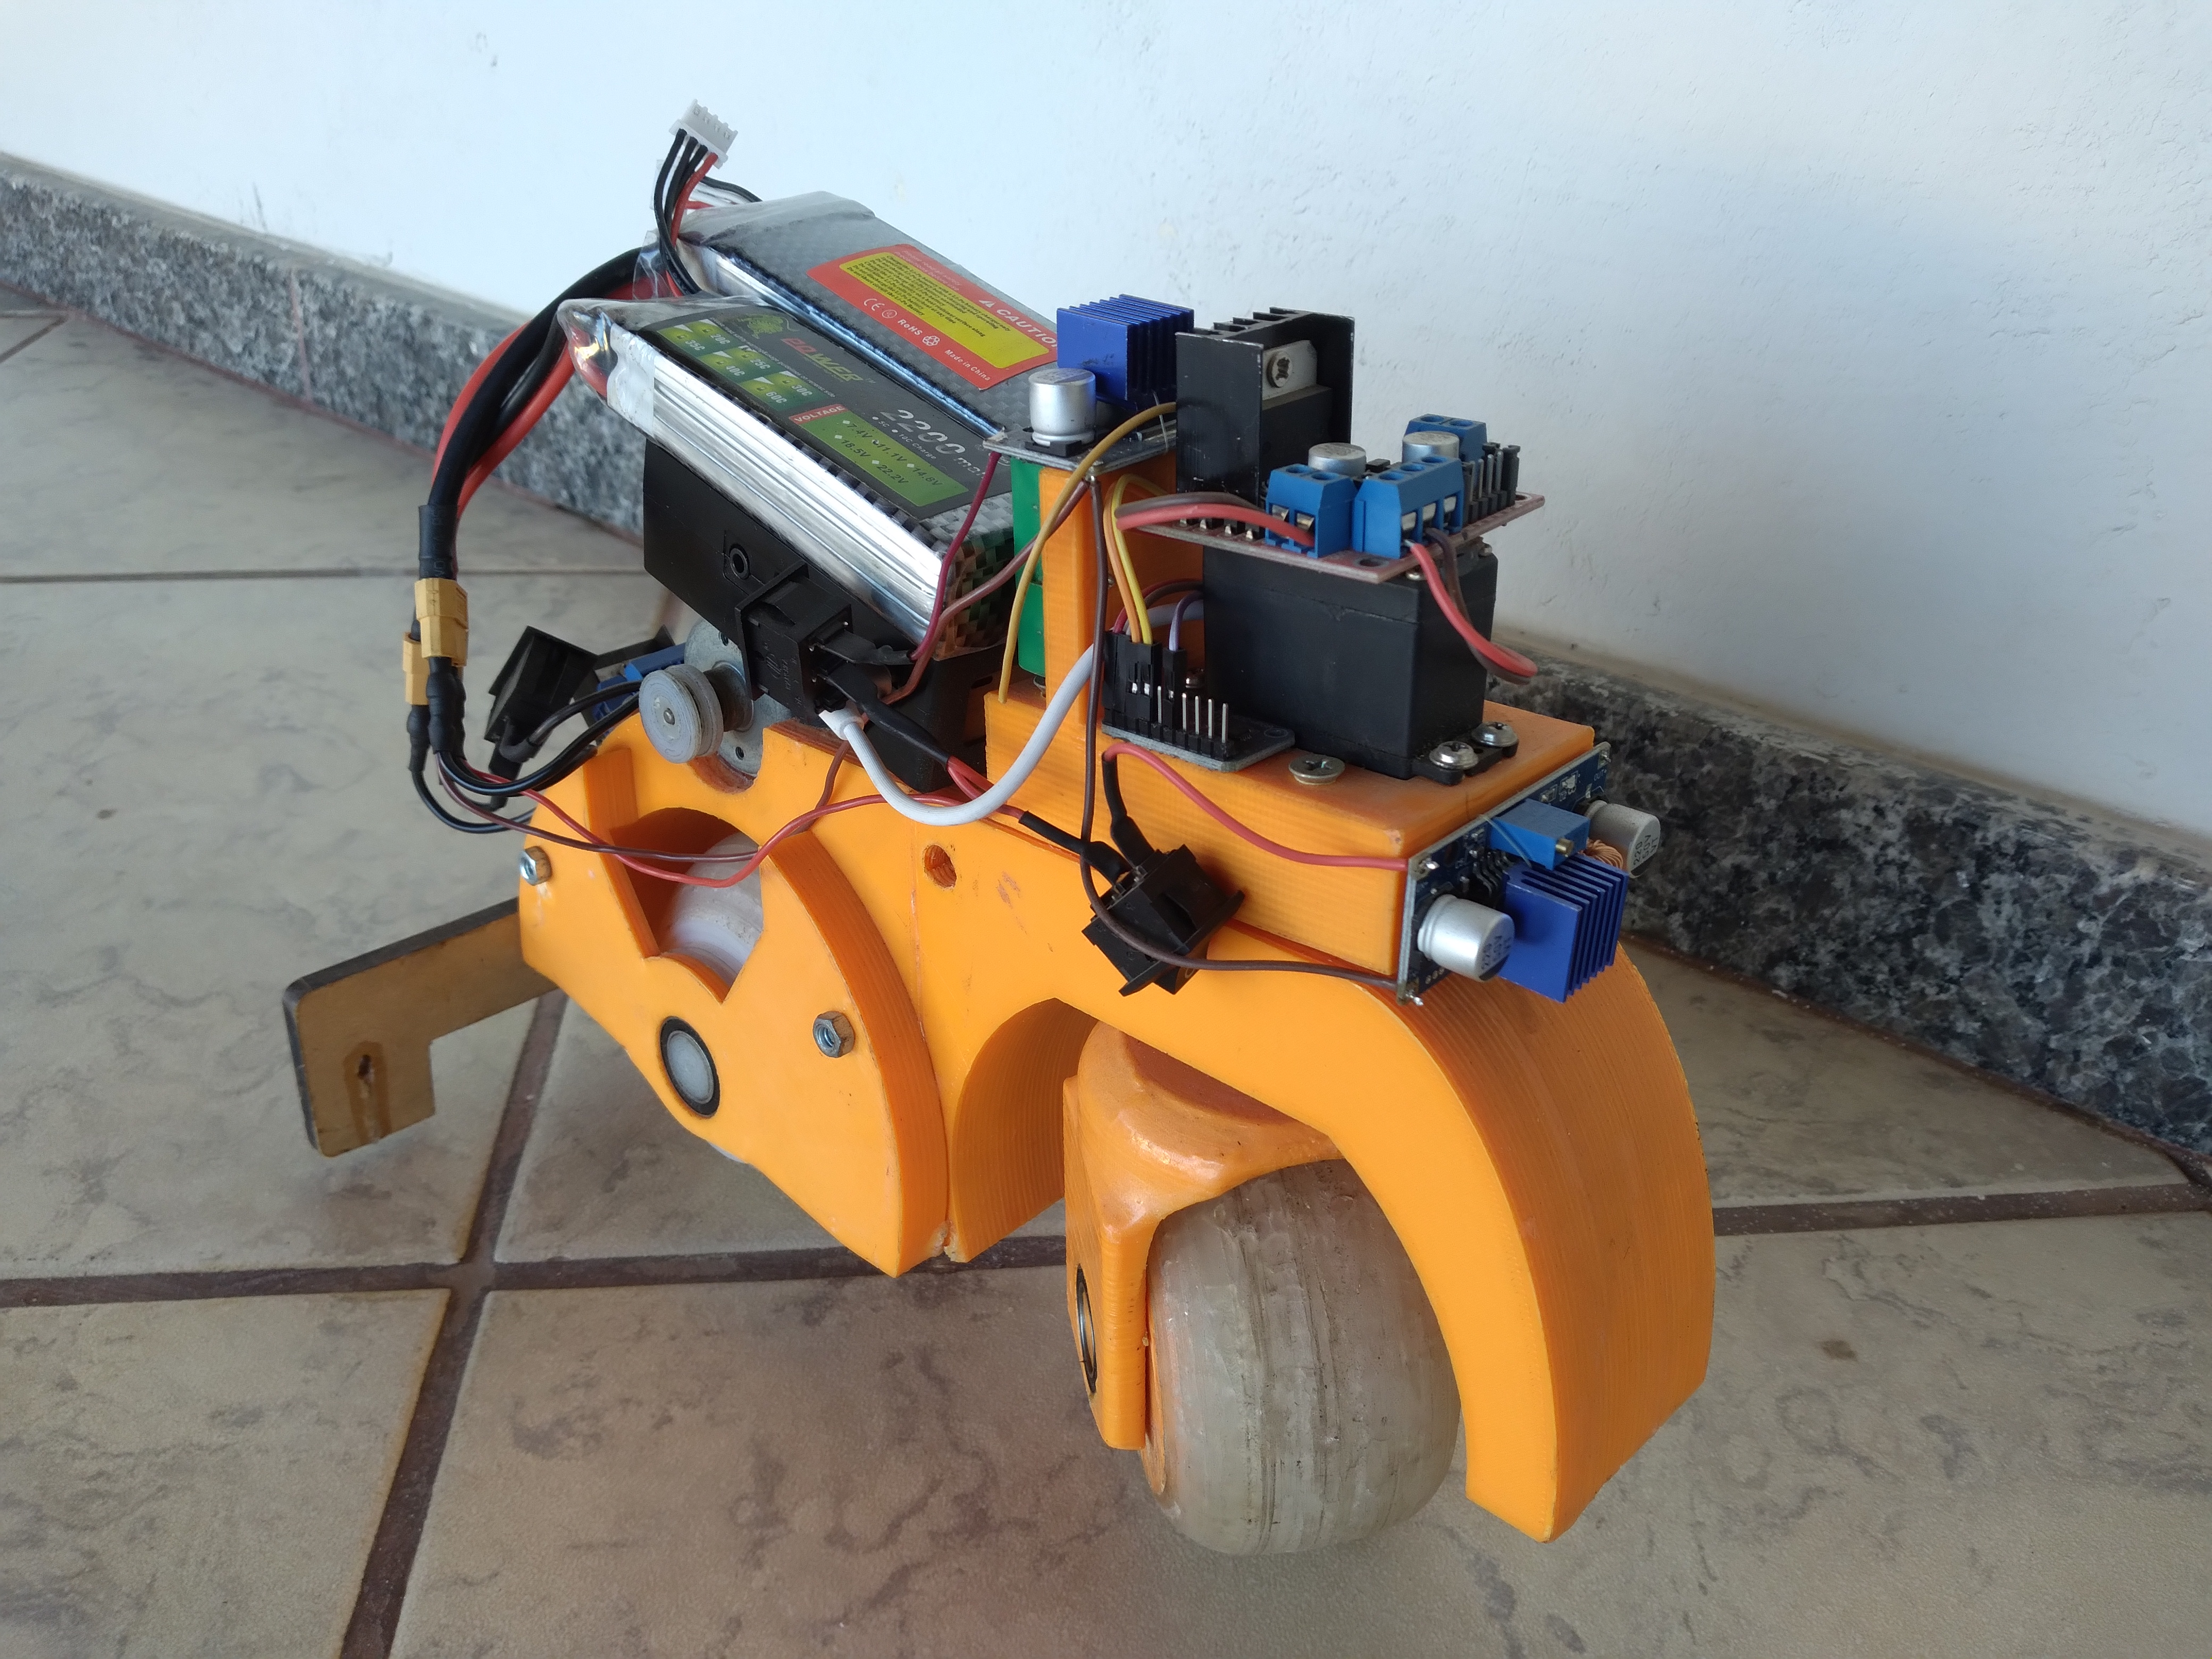
\includegraphics[width=13cm]{Imagens/MotinhaIsometricaDianteira.jpg}{%\columnwidth
                \small
                \centering
                \caption{Vista Isométrica Dianteira da Planta}
                \label{fig:motinha1}}
        \end{figure}
        
        \begin{figure}[!htb] 
            \centering
            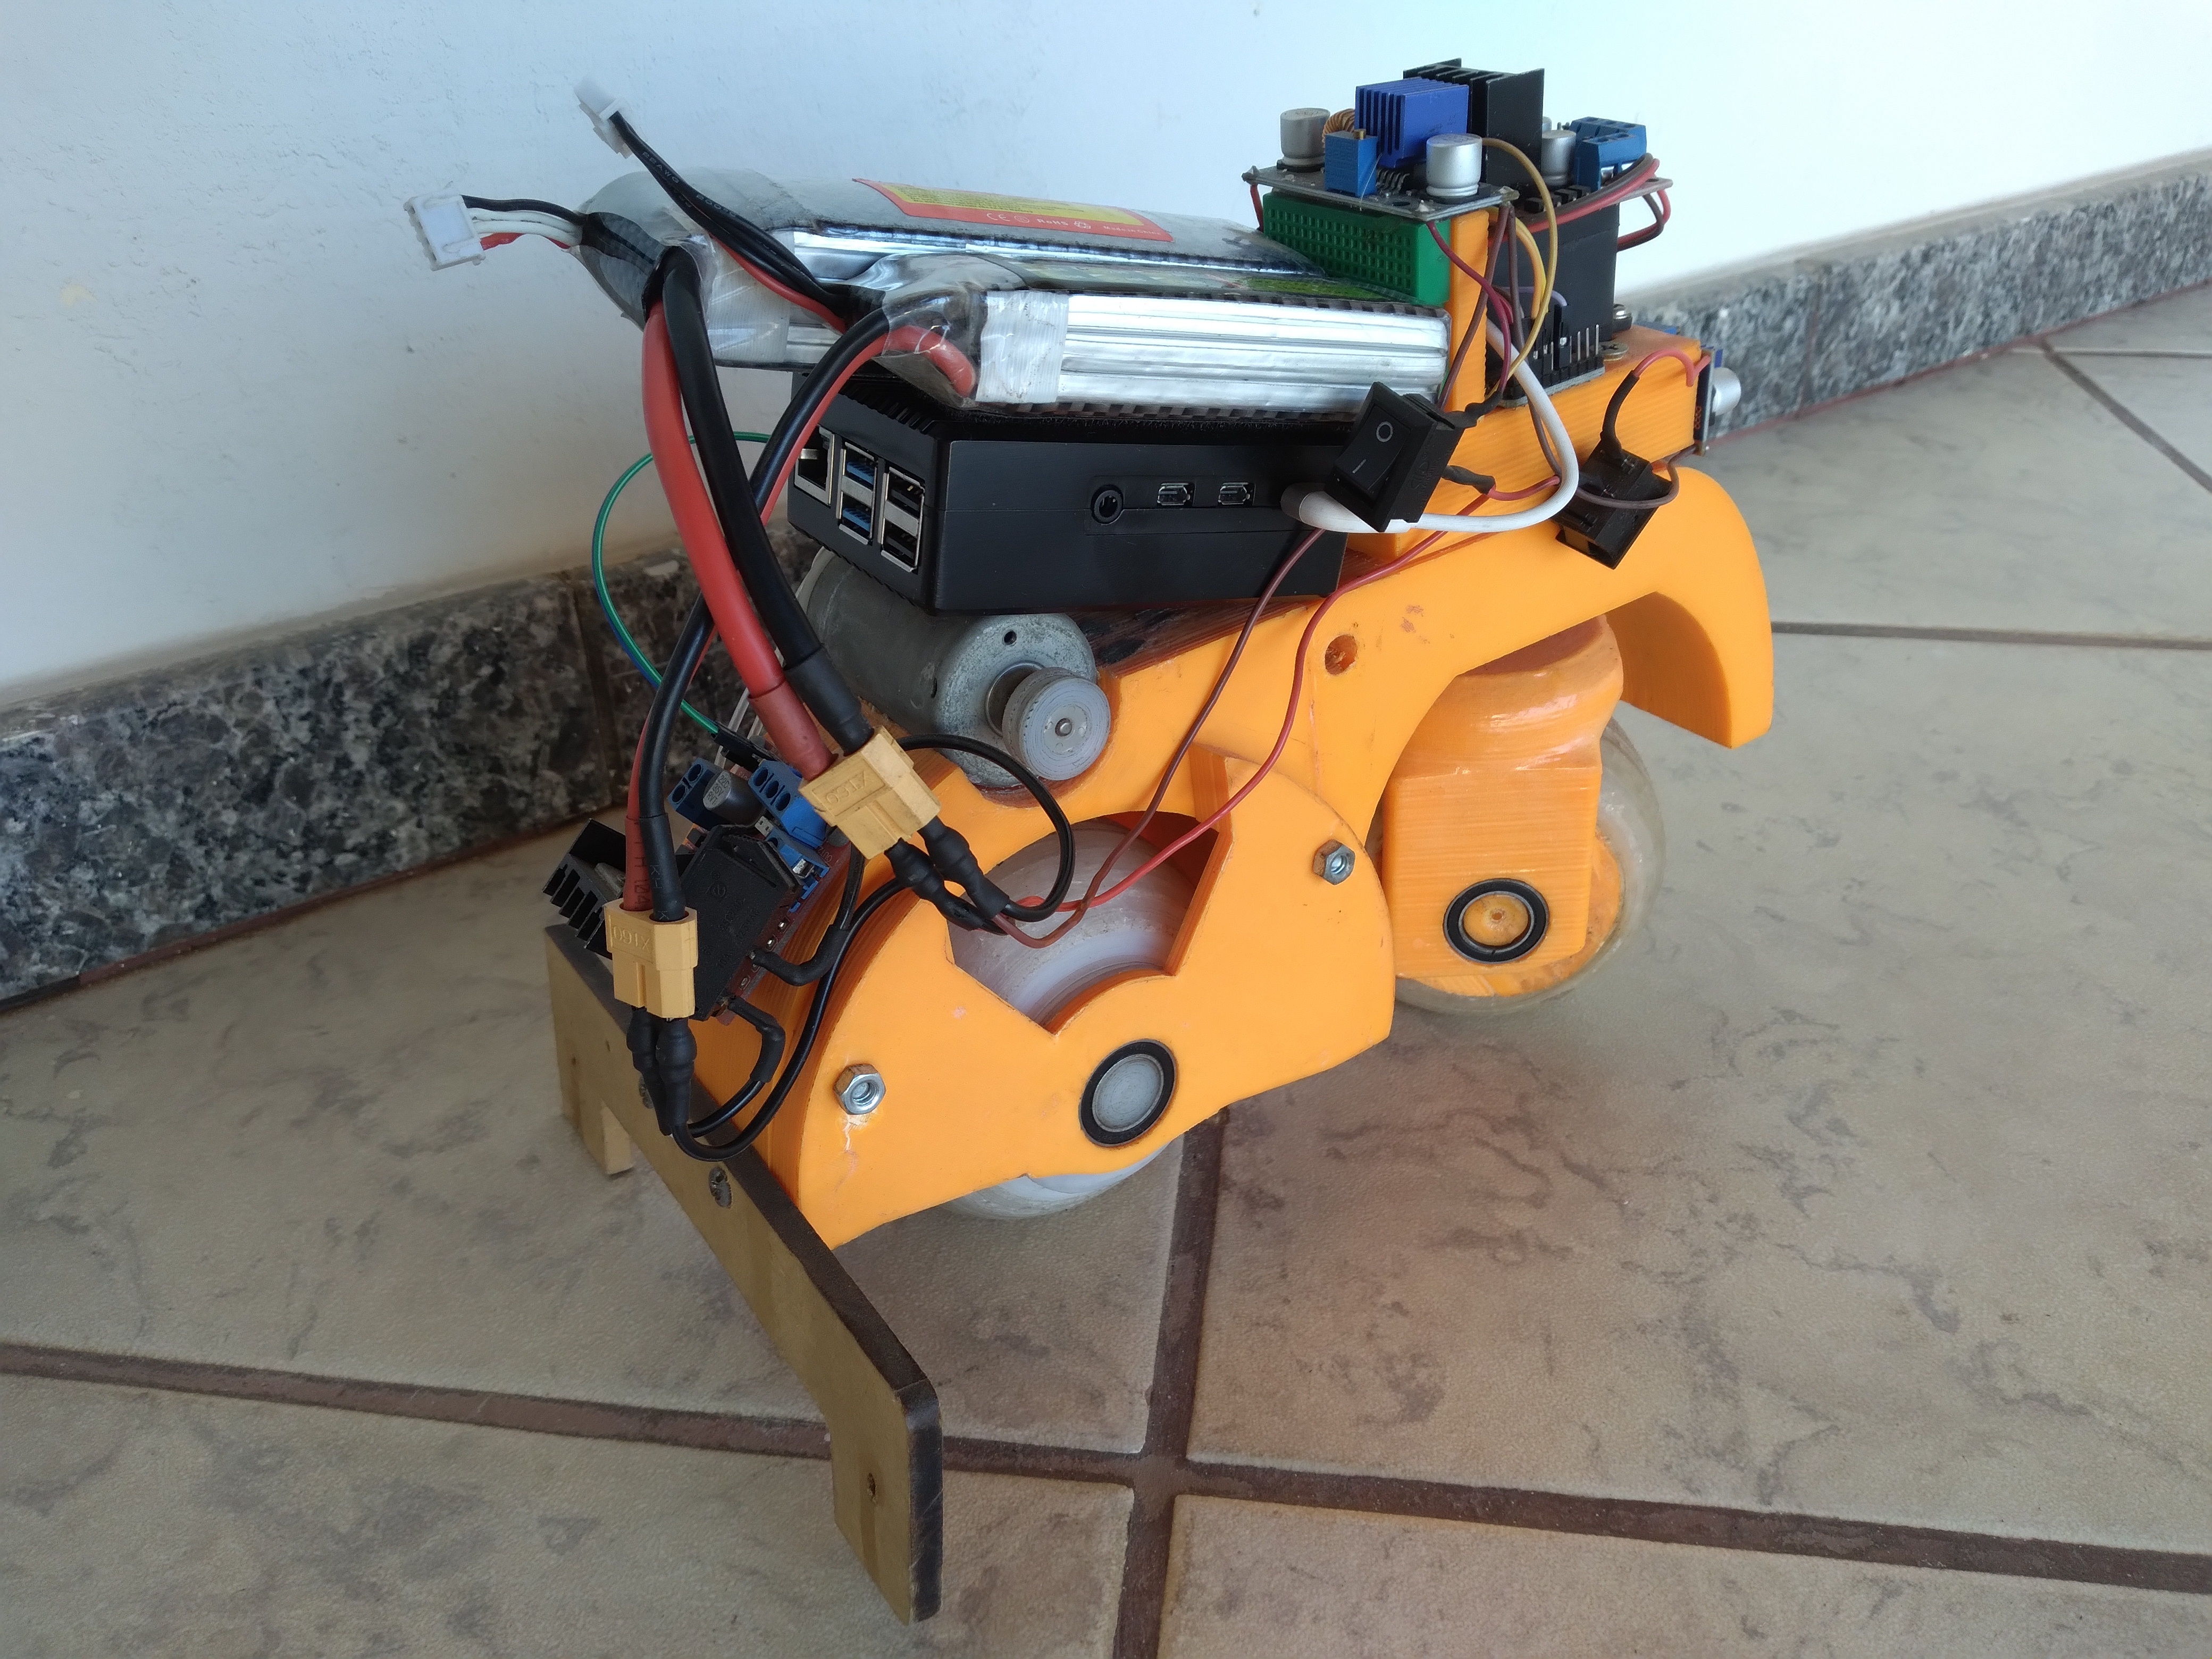
\includegraphics[width=13cm]{Imagens/MotinhaIsometricaTraseira.jpg}{
                \small
                \centering
                \caption{Vista Isométrica Traseira da Planta}
                \label{fig:motinha2}}
        \end{figure}
		
	\section{Hipótese}
	    %Hipótese
	    Parte-se da hipótese que é possível equilibrar uma bicicleta apenas alterando a direção do eixo de direção, sem deslocamento de massa e consequentemente, do centro de gravidade, mas com um atuador acoplado no eixo de direção que cancela o sistema mecânico de equilíbrio da bicicleta. Assim, para viabilizar o teste da hipótese, realiza-se uma pesquisa de finalidade aplicada, objetivo exploratório, sob o método hipotético-dedutivo, com abordagem quantitativa, realizada com procedimentos experimentais. %Metodologia
        
    \section{Objetivos} %Objetivo geral     %Objetivos Específicos
        
        O objetivo geral do trabalho é investigar a controlabilidade e sintetizar controladores que possam estabilizar o pendulo invertido em torno da posição de equilíbrio, caso este sistema seja controlável. 
		
		\subsection{Objetivos específicos}
		    Para atingir o objetivo geral, é necessário antes atender outras metas, como:
            \begin{itemize} %O ideal é que cada objetivo especifico se torne um capítulo do TCC
                \item Modelar matematicamente os sistemas da planta de controle;
                %\item Obter os parâmetros para o modelo.
                %\item Criar um modelo computacional baseado no modelo matemático e nos parâmetros obtidos. 
                \item Sintetizar controladores para os modelos obtidos;
                \item Desenvolver um software para aplicar os controladores na planta de controle.
            \end{itemize}
        
	\section{Organização do texto}  %Previa dos capítulos        %Hipótese        %Previa conclusão
	    
	    %Previa de Fundamentos
	    O capítulo \ref{chp:fundamentos} apresenta a revisão teórica necessária para desenvolver a modelagem do sistema.  %apresenta o referencial teórico do tema e a referência bibliográfica dos assuntos tratados.
	    
	    O capítulo \ref{chp:Hardware} apresenta os componentes elétricos e eletrônicos da planta, bem como a integração entre eles.
	    
	    %Previa de Modelagem do sistema
	    Já o capítulo \ref{chp:modelagem} apresenta a modelagem dinâmica do subsistema de velocidade tangencial, do subsistema do ângulo de direção e do subsistema do pendulo invertido, que é dividido na modelagem cinemática da aceleração e a modelagem da dinâmica de bicicleta.
	    
	    %Previsão de TCC2
	    São previstos dois capítulos a serem escritos durante a execução da disciplina de TCC 2. No caso o capítulo \ref{chp:Hardware} passará a ser chamado de "Hardware e Software", onde será apresentado também a metodologia e desenvolvimento do software, e um novo capítulo chamado "Sintase de Controladores" onde será dissertado sobre a metodologia, síntese e o resultados dos controladores aplicados a planta.
	    
	    %Conclusão
	    Ao final deste trabalho conclui-se no capítulo \ref{chp:conclusão} que o objetivo de modelar os sistemas da planta foi atingido, ficando o restantes dos objetivos e a confirmação (ou não) da hipótese planejados para o desenvolvimento de TCC2.
	    
	    %Tarefas
	    %Revisão de Literatura
	    %Capitulo hardware
	    %Cronograma
	    %Resumo
	    